\documentclass[12pt,addpoints,answers]{guia}
\grado{3$^\circ$ de Secundaria}
\cicloescolar{2022-2023}
\materia{Ciencias y Tecnología: Química}
\guia{26}
\unidad{3}
\title{Reconvinaciones atómicas}
\aprendizajes{
    \begin{itemize}[leftmargin=*,label=\small\color{colorrds}\faIcon{user-graduate}]
        \item Argumenta acerca de posibles cambios químicos en un sistema con base en evidencias experimentales. 
        \item Reconoce y valora el uso de reacciones químicas para sintetizar nuevas sustancias útiles o eliminar sustancias indeseadas. 
        \item Reconoce la utilidad de las reacciones químicas en el mundo actual.
        \item Explica, predice y representa cambios químicos con base en la separación y unión de átomos o iones, y se recombinan para formar nuevas sustancias.
    \end{itemize}
}
\author{JC Melchor Pinto}
\begin{document}
\pagestyle{headandfoot}

\INFO
\printanswers
\begin{multicols}{2}
    \include*{../blocks/block0000}
\end{multicols}
% \begin{opening}[Atracción electrostática]
%     {Objetivo:\\ Observar el comportamiento de diferentes sustancias ante la presencia de un objeto
%         con carga eléctrica.

%         \begin{minipage}{0.3\textwidth}
%             \begin{figure}
%                 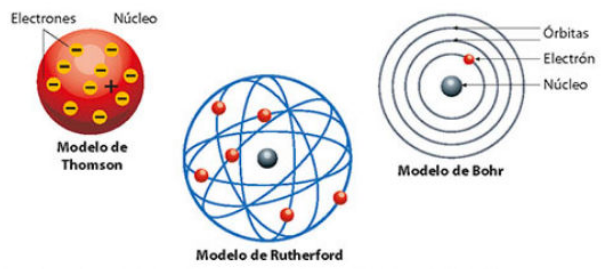
\includegraphics[width=0.9\linewidth]{atomicsmodels}
%                 \caption{Imagen ejemplo del experimento}
%                 \label{fig:}
%             \end{figure}

%         \end{minipage}\hfill
%         \begin{minipage}{0.6\textwidth}
%             Materiales:
%             \begin{itemize}
%                 \item Globo o varilla de plástico o vidrio
%                 \item Franela
%                 \item Bureta o jeringa de 10 mL
%                 \item Vaso de precipitados o de plástico
%                 \item Soporte universal
%                 \item Pinzas de laboratorio
%                 \item Diferentes sustancias líquidas (agua, etanol, acetona, hexano).
%             \end{itemize}

%             Procedimiento:
%             \begin{enumerate}
%                 \item Froten el globo o la varilla de plástico o vidrio con una franela para cargarlo eléctricamente.
%                 \item Predigan, antes de realizar el experimento, si el objeto cargado atraerá, repelerá o no afectará el chorro de cada líquido. Justifiquen sus ideas.
%                 \item Sujeten la bureta al soporte y abran la llave para que salga un chorro de agua delgado, pero continuo.
%                 \item Acerquen el objeto cargado al chorro de agua sin tocarlo. ¿Qué sucede?
%                 \item Repitan el experimento con otros líquidos (etanol, acetona, hexano).
%             \end{enumerate}

%             Análisis de resultados y conclusiones:
%             \begin{enumerate}
%                 \item Contrasten los resultados con sus predicciones.
%                 \item Generen hipótesis iniciales que expliquen por qué los líquidos que utilizaron se comportan de diferente manera.
%             \end{enumerate}
%         \end{minipage}
%     }
% \end{opening}
% \begin{multicols}{2}
% \include*{../blocks/block030a}
% \include*{../blocks/block030b}
% \end{multicols}
\begin{questions}
    \question
    % \include*{../questions/question067a}
    % \include*{../questions/question068a}
\end{questions}
\end{document}